\documentclass[conference]{IEEEtran}
\usepackage{graphicx}
\begin{document}
\title{Word Hunter}
\author{\IEEEauthorblockN{Yang Zhao}
\IEEEauthorblockA{yzhao3@stanford.edu}
\and
\IEEEauthorblockN{Shuo Liu}
\IEEEauthorblockA{shuol@stanford.edu}
\and
\IEEEauthorblockN{Lingren Zhang}
\IEEEauthorblockA{lz7@stanford.edu}
}

% make the title area
\maketitle


\begin{abstract}
For this project we propose and implement a reading tool on Andriod platform that can be used to identify keywords on paper-based media.  After receiving an image of the media, we first pre-process the image (binarization and de-skew), and then use OCR (in particular, Tesseract OCR engine) to recognize the text and find the keywords, at last we highlight the keywords by circling it with a red box.
\end{abstract}

\section{Introduction}
Have you ever read a long paper-based article and find yourself unable to locate keywords? With the advancement of digital media, sometimes we take basic word search for granted. But the world is still full of media printed on paper and it would make our lives much simpler if we can automate this basic reading tool for good old fashioned books. We propose a mobile application that will be able to find a word that the user specified through a phone’s viewfinder. As soon as the phone detects the word it will highlight it, saving the user many minutes of looking for the word him/herself. 

For example, we want to search for “nonlinear equation” in this page of paper. We only need to use our smart phone to scan over the paper. Whenever the word “nonlinear equation” appears on the phone screen, it will be immediately circled in red.\\

\begin{figure}
\center
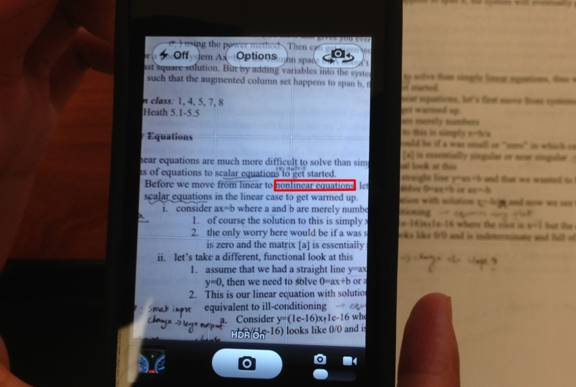
\includegraphics[scale=0.5]{demo.jpg}
\caption{Word Hunter Demo}
\end{figure}

\section{Preprocessing}
\subsection{Binarization}

The first step is to apply locally adaptive thresholding algorithm in order to separate text from background in a grayscale image (which can be derived from RGB).  The reason we choose locally adaptive thresholding instead of global thresholding is that the lighting/brightness of the image is not uniform which will cause global thresholding to perform poorly in the extreme bright/dark regions.

The idea of locally adaptive thresholding is divide the image into blocks/windows.  For each block, use grayscale variance to determine whether the block is uniform.  If the block is non-uniform (high variance), apply Otsu's method/global thresholding to the block; if the block is uniform (low variance), classify the entire block as all black or all white based on the mean grayscale value.  The reason not to apply Otsu's method to every block is because some blocks maybe entirely background with a number of noise pixels, Ostu's method will keep the noise pixels while classifying the entire block as background will eliminate noise.

We applied OpenCV function adaptiveThreshold for binarization.  We also observed that a blockSize of 41 yields the best thresholding result.  See Figure~\ref{noskew} and Figure~\ref{noskewbinarized} for an example of image before and after binarization.

\begin{figure}
\center
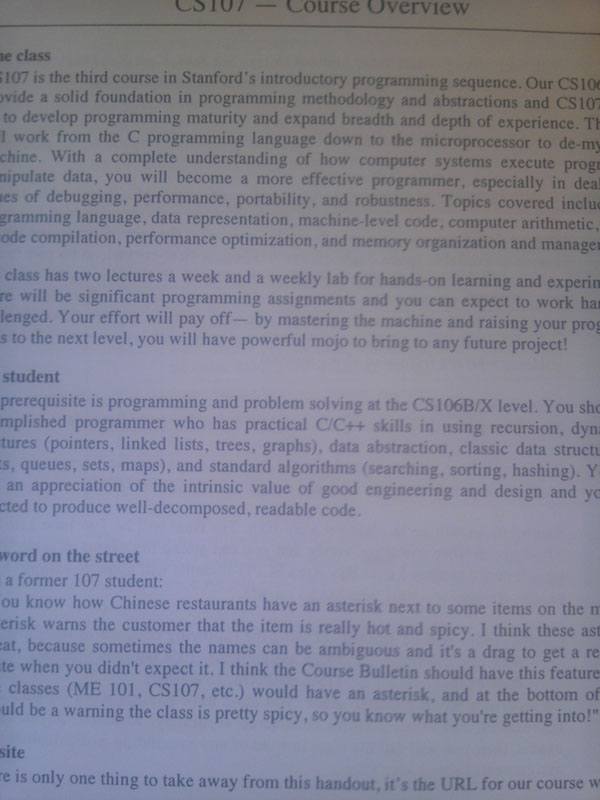
\includegraphics[scale=0.25]{no_skew.jpg}
\caption{Before Binarization}
\label{noskew}
\end{figure}

\begin{figure}
\center
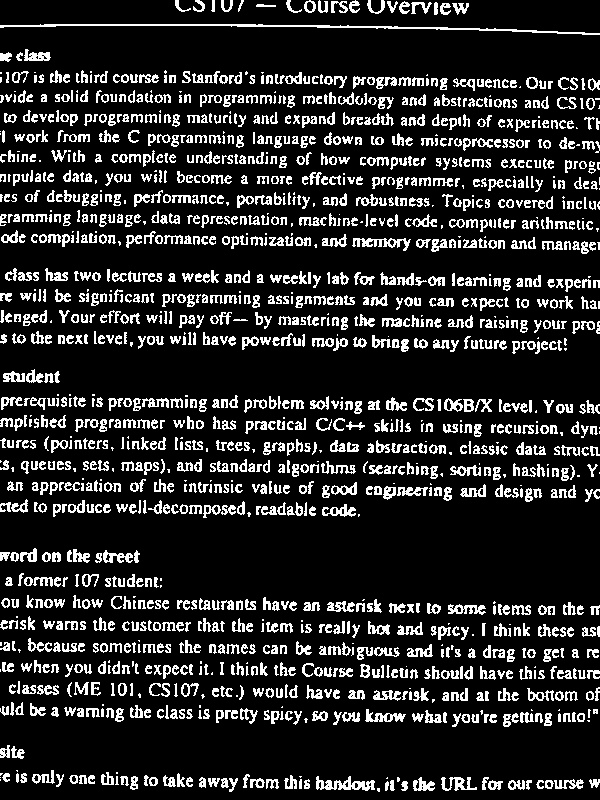
\includegraphics[scale=0.25]{no_skew_binarized.jpg}
\caption{After Binarization}
\label{noskewbinarized}
\end{figure}

\subsection{De-skew}

Hough transform (OpenCV function HoughLinesP) is used to detect (text) lines in the image.  Then we rotate binarized image by the mean of the rotation angles calculated from each text line, we call OpenCV function getRotationMatrix2D to do it.  We also need to make sure not to cut off corners in the rotation process, therefore we need to pad the binarized image before rotating.  See Figure~\ref{binarized} and Figure~\ref{deskewed} for an example of image before and after de-skew.  Notice that Figure~\ref{deskewed} is slightly larger because of padding.

\begin{figure}
\center
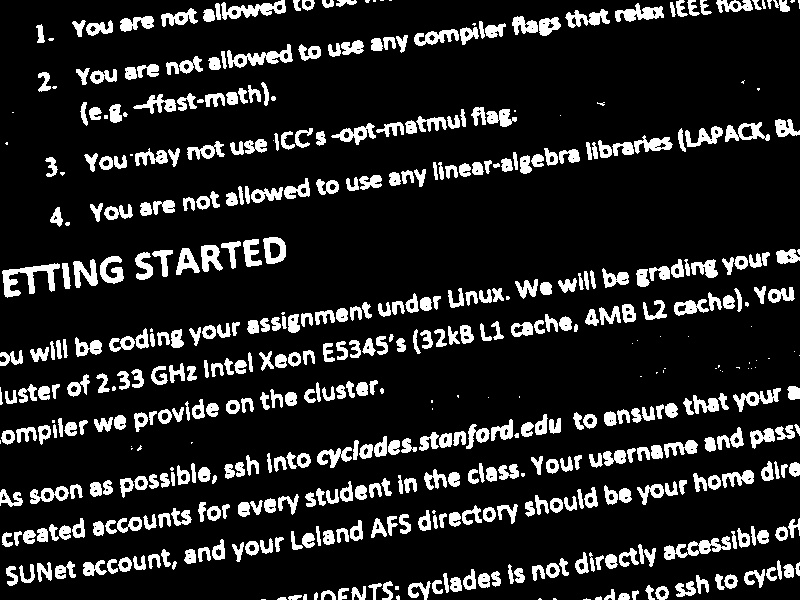
\includegraphics[scale=0.15]{binarized.jpg}
\caption{Binarized Image Before Deskew}
\label{binarized}
\end{figure}

\begin{figure}
\center
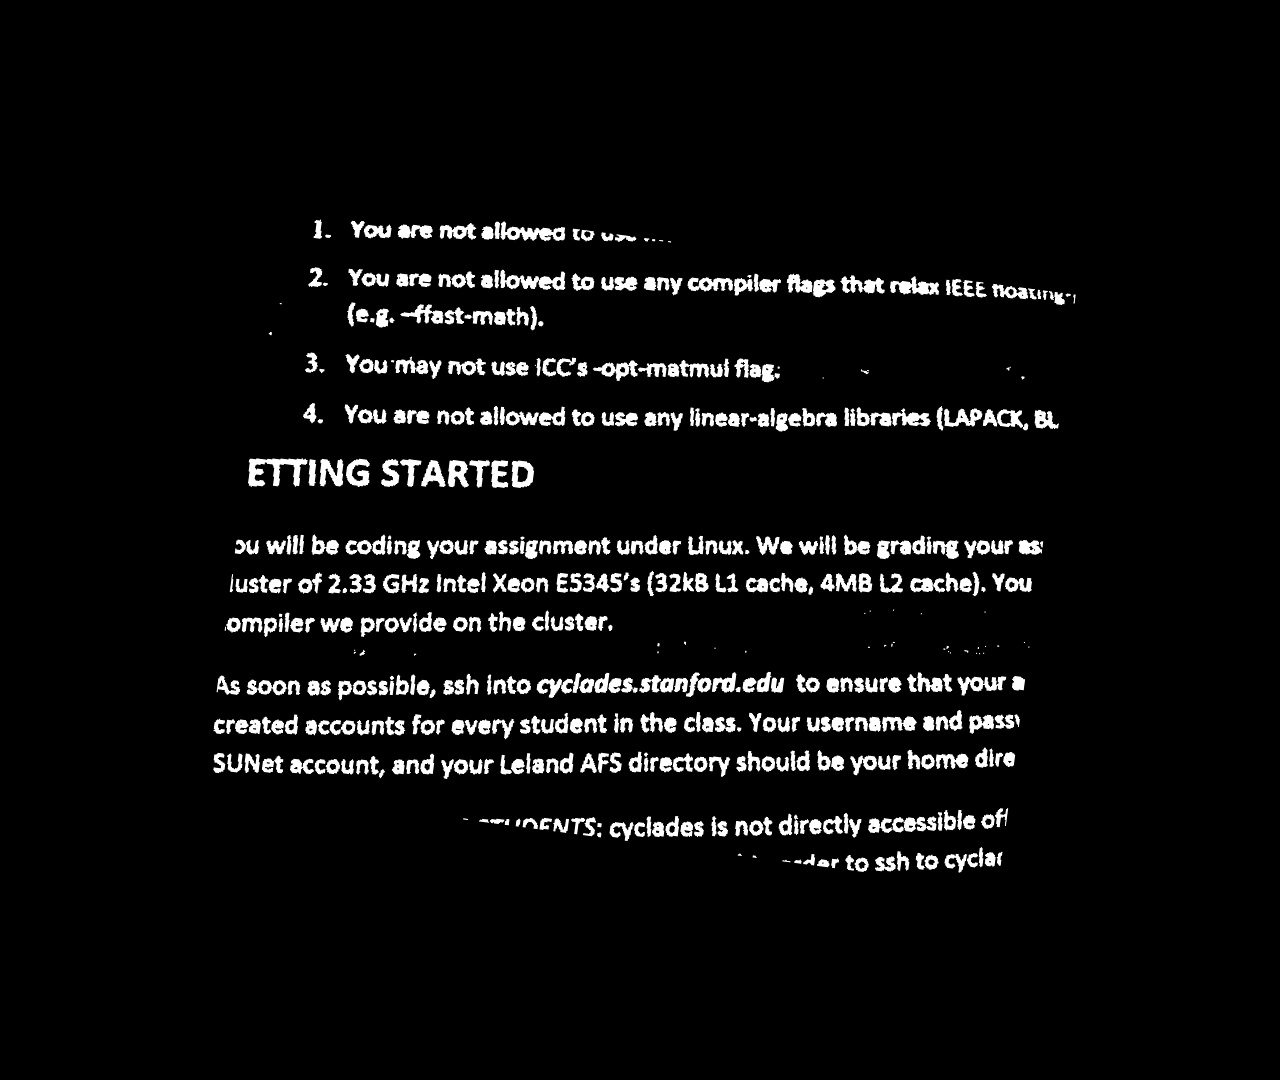
\includegraphics[scale=0.15]{deskewedImage.jpg}
\caption{Binarized And Deskewed}
\label{deskewed}
\end{figure}

\section{Word Recognition}

\subsection{Segmentation By Letter}
The first step of word recognition is to segment the image into rectangles each containing a letter.  Because most letters consists of one connected component in the image, we can draw a contour (OpenCV function findContours and drawContours) around each letter and then find a bounding box of each contour (OpenCV function boundingRect). See Figure~\ref{letterbbox} for an example of each letter surrounded by a rectangular bounding box.

Some letters (for instance, lower case ``i'', ``j'') consists of two connected components, and hence will have two bounding boxes, but it doesn't affect the algorithm as they will get combined in the next step as we combine letter bounding boxes into word bounding boxes.  

\begin{figure}
\center
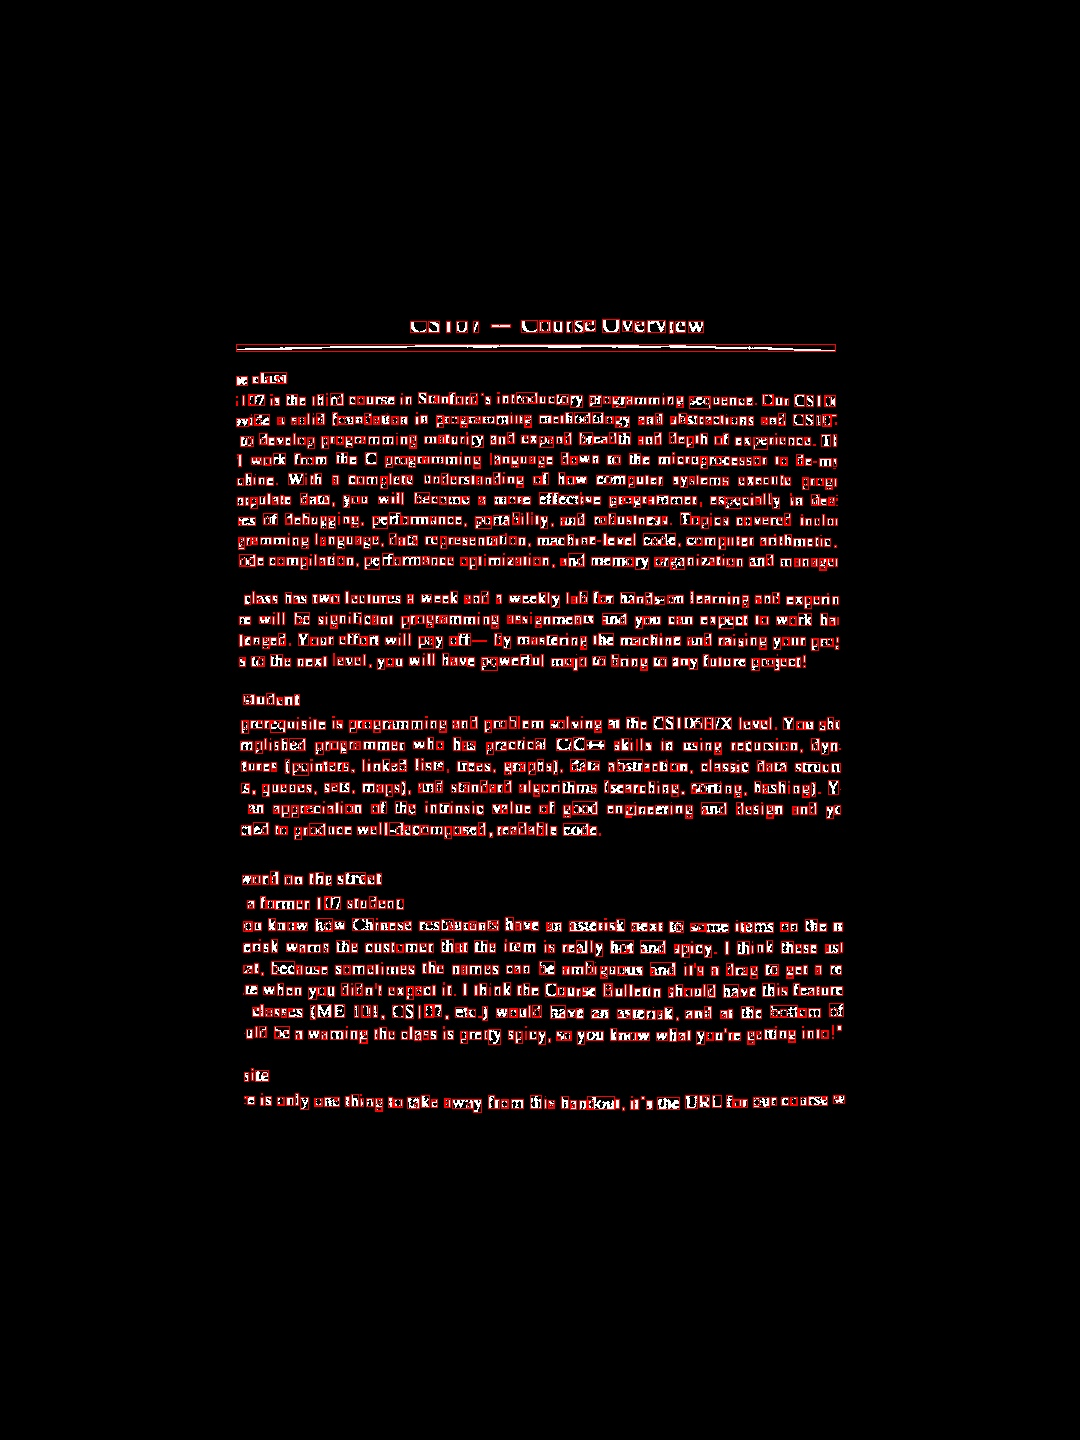
\includegraphics[scale=0.15]{letter_with_bounding_box.jpg}
\caption{Segmentation By Letter}
\label{letterbbox}
\end{figure}

\subsection{Segmentation By Word}

In this step, we need to combine neighbouring letter bounding boxes into a word bounding box, but there is no existing OpenCV functions that performs this task.  We implemented the three functions below in C++:

\subsubsection{Find Character Size}
We implemented function findCharSize to estimate the average height and width of each letter (or its bounding box).  

\subsubsection{Find Neighbour}
We implemented isNeighbour to determine where two letters are next to each other in the same word.

\subsection{Tesseract}
findEditDistance

\section{Server Client Connection}

\section{Conclusion}

\section*{Acknowledgment}
We would like to thank David Chen and Sam Tsai for their generous and responsive help on the project.


%\begin{thebibliography}{1}
%\bibitem{IEEEhowto:kopka}
%H.~Kopka and P.~W. Daly, \emph{A Guide to \LaTeX}, 3rd~ed.\hskip 1em plus
%  0.5em minus 0.4em\relax Harlow, England: Addison-Wesley, 1999.
%\end{thebibliography}

\end{document}